\documentclass[12pt,a4paper,titlepage]{article}
%\documentclass[12pt, a4paper, UTF8]{ctexart}
\usepackage{CJK}

\usepackage{ctex}
\usepackage{lipsum}     %随机生成文本的宏包
\usepackage{geometry}   %设置页边距的宏包
\usepackage{titlesec}   %设置页眉页脚的宏包
\usepackage{setspace}   %行距
\usepackage{fancyhdr}	   %页眉页脚  
%\usepackage{titlesec}   %设置子标题字体
\usepackage{titlesec}
\usepackage[colorlinks,linkcolor=black]{hyperref}  %超链接
\usepackage{epsfig}           %插图
\usepackage{graphicx}
\usepackage{subfigure}
\usepackage{enumitem}
\usepackage{amsmath}          %split
\usepackage{listings}    %代码环境

%说明。bibtex如果需要引用中文文献,编码方式要一致,否则乱码,我的是使用utf-8无签名就不会乱码。

\setCJKmainfont{宋体}   %全局中文环境

\setenumerate[1]{itemsep=0pt,partopsep=0pt,parsep=\parskip,topsep=5pt}
\setitemize[1]{itemsep=0pt,partopsep=0pt,parsep=\parskip,topsep=5pt}
\setdescription{itemsep=0pt,partopsep=0pt,parsep=\parskip,topsep=5pt}

\titleformat{\paragraph}[block]{\normalsize\bfseries}{\theparagraph}{1em}{}  %paragraph 换行


\titleformat{\section}%设置section的样式
{\center\zihao{-2}\bfseries}%右对齐,小二号字,加粗
{\thesection .\quad}%标号后面有个点
{0pt}%sep label和title之间的水平距离
{}%标题前没有内容

\titleformat{\subsection}%设置section的样式
{\raggedright\zihao{-3}\bfseries}%右对齐,小三号字,加粗
{\thesubsection.\quad}%标号后面有个点
{0pt}%sep label和title之间的水平距离
{}%标题前没有内容

\titleformat{\subsubsection}%设置section的样式
{\raggedright\zihao{4}\bfseries}%右对齐,四号字,加粗
{\thesubsubsection.\quad}%标号后面有个点
{0pt}%sep label和title之间的水平距离
{}%标题前没有内容 

\newcommand{\upcite}[1]{\textsuperscript{\textsuperscript{\cite{#1}}}}  %引用右上角


\pagestyle{fancy}
\fancyhf{}
\setlength{\baselineskip}{18pt}
\geometry{left=3cm,right=2.5cm,top=2.5cm,bottom=2.5cm}  %设置 上、左、下、右 页边距



\cfoot{\zihao{5} \thepage}
\fancyhead[CO,CE]{\zihao{4} 安徽工业大学毕业设计}


\title{基于深度卷积神经网络和迁移学习的行人检测算法探究与实现}
\author{吴若晨}
\date{\today}




\begin{document}




\renewcommand{\figurename}{图}
\maketitle

\renewcommand{\abstractname}{\zihao{3} 摘要}
\begin{abstract}
\qquad 行人检测,是利用计算机视觉技术在静态图像或动态视频序列中,查找并定位行人的算法。由于其应用方向广,挑战难度大,所有学术工业界均有着深入的研究。
传统行人检测算法,如Hog+SVM法,主要使用如下流程:提取静态特征(边缘特征,统计特征等),滑动窗口分类行人,但传统算法仍有许多不足:对模糊图像识别效果差,不能准确定位,漏识别,错识别概率高。\par
自Alexnet于2012年在ImageNet竞赛大放异彩开始,深度学习开始受到人们的广泛关注。其中深度卷积神经网络,由于其强大的特征提取特性,在计算机视觉各个方面上,都对传统方法实现了超越。各种多类物体检测算法在深度学习的帮助下都实现了质的突破。
另一方面,深度卷积网络对数据集要求非常高,很多算法都是在小数据集上没法训练出令人满意的结果,所以研究人员通常采用的是迁移学习中微调的技术,首先在大型数据集上(如ImageNet)进行预训练,之后在得到的网络模型上再使用自身数据集进行训练,这样往往能够保证效果。\par
本毕设的构想是通过复现基于深度卷积网络的几个物体检测算法,如Faster-RCNN,YOLO,SSD,利用微调技术,将它们迁移至行人检测任务上来,并期望相较迁移学习前的算法,行人检测部分性能有所提升。
\begin{center}
{\textbf{关键词}:卷积神经网络,物体检测,迁移学习,行人检测}
\end{center}
\end{abstract}

\renewcommand{\abstractname}{\zihao{3} Abstract}
\begin{abstract}
\qquad Pedestrian detection is an algorithm to find and locate pedestrians in static image or dynamic video sequences using computer vision technology.
Because of its wide application prospect and great challenge, both Academia and Industry have much research on it.
The traditional pedestrian detection algorithm, such as Hog+SVM method,mainly follows these two steps:
extracting static features (edge feature, statistical feature etc), using sliding window to classify pedestrians.Still there are a good many deficiencies of traditional algorithms.
They have problem with processing fuzzy pedestrain, fail to precisely localize, and have a high error of wrong detection.\par
Since 2012 when AlexNet yields unusually brilliant results in the ImageNet competition,people have been arousing great interests in deep learning.
Meanwhile deep convolutional nerual network has surpassed the traditional methods in many aspects of computer vision due to its excellent ability of extracting features.
On the other hand, convolutional neural networks require large amounts of data, algorithm usually fails to work when training in small scale dataset.
To deal with it, reasearchers generally use the method fine-tuning,which is one of the effective way of transform learning.
First pre-train their model in the large data set (such as ImageNet) , then use their own data set(much smaller) to train, this strategy often effects.\par
This graduation project aims at reimplementing several state-of-art object detection algorithm, such as Faster-RCNN, YOLO, SSD, and transforming them to the task of pedestrain detection using the technology of fine-tuning.
Besides compared to the original object detection algorithm, these transformed method should perform better in this specific detection of pedestrain.
\begin{center}
{\textbf{keywords}: CNN, object detection, tranform learning, pedestrain detection}
\end{center}
\end{abstract}

\renewcommand{\contentsname}{目录}
\tableofcontents
\newpage

\section{绪论}
\subsection{研究背景及意义}
\subsubsection{研究背景}


行人检测作为计算机视觉中的一个经典的主题,其在学术界和工业界一直有着广泛的研究和应用。现有的行人检测方法主要为一些非深度方法,这些方法进一步又可分为基于背景建模的方法和基于机器学习的方法。背景建模法通过建立背景模型,利用背景减分割出前景,进一步判断和提取其中的行人目标。这类方法的抗干扰能力不强,难以处理背景的动态变化以及摄像头运动下拍摄的动态场景。而机器学习的方法则可归纳为特征工程结合分类器,首先使用一系列手工特征的组合,如Integral channel features\upcite{dollar2009integral},HoG\upcite{dalal2005histograms}以及它们的变体\upcite{felzenszwalb2010object,schwartz2009human},再将这些提取的特征送入诸如SVM\upcite{felzenszwalb2010object},随机森林\upcite{dollar2012crosstalk}等分类器进行训练与测试。相较于背景建模的方法,机器学习方法对动态场景有着更强的鲁棒性和更低的误检率。然而,由于受限于浅层特征的表达能力,传统基于机器学习的行人检测算法,往往泛化能力较差,如果适用的场景与训练数据集差异很大,则这些方法的性能会急剧下降。为了解决问题,需要重新采集和标注大量的数据样本,耗时耗力,且若场景再次切换,需要重复如上工作。关于如何解决这个问题,学术界也对相应的机器学习方法细节进行了改进。然而正如机器学习工业界广为流传着的这样一句话:“数据和特征决定了机器学习的上限,而模型和算法只是逼近这个上限而已”,所以挖掘更高层次的特征,是解决检测问题一大重要方向。\par
另一方面,深度学习曾作为神经网络被我们广为熟知,在20世纪80年代流行过一阵,取到了相对较小的成功。然而在之后的几年里,神经网络被许多其他方法超越。神经网络训练慢,并且就深度神经网络从一个随机生成的权重起点开始训练是否可行,学术界没有达成广泛的一致,渐渐地被研究人员抛弃。现如今随着与日俱增的数据量和不断增强的计算力,我们拥有的计算资源可以运行更大的模型,深度学习的精确识别和预测能力也一直在提高。深度卷积神经网络作为深度学习的一个子集,具有强大的特征提取能力,而这一特性,恰好适合计算机视觉中各类图像任务。关于深度学习能力的一个粗略的经验法则是:监督深度学习算法在每类给定约5000个标注样本情况下一般将达到可接受的性能,当至少有1000万个标注样本的数据集用于训练时,它将达到或超过人类表现\upcite{Goodfellow-et-al-2016}。深度学习随着卷积网络AlexNet\upcite{krizhevsky2012imagenet}在ImageNet竞赛大放异彩而迅速崛起,随后卷积网络在图像识别\upcite{simonyan2014very,he2016deep},物体检测\upcite{ren15fasterrcnn,redmon2016you,liu2016ssd}等各个方向实现了对传统方法的超越。特定到行人检测的深度学习方法,也有相关的研究\upcite{sermanet2013pedestrian}。关于神经网络和卷积网络的相关概念,可参考本毕业设计于附录A部分的简单介绍。

本课设旨在从深度学习中卷积神经网络的角度切入,改善非深度方法中对模糊图像处理乏力,泛化能力不强的缺陷。并相较传统方法,达到更高的准确率,和更低的漏检,错检率。 
\subsubsection{研究意义}
行人检测作为计算机视觉长久以来的热门话题,其早已有着实际应用,在智能交通领域,行人检测可作为人流量统计的技术辅助手段,在自动驾驶领域,行人检测同样是关键的一环。在视频监控领域,从针对切割图像的行人重识别(Re-ID)技术扩展到针对全景图像的算法行人搜索(Person Search),这其中的关键,正是行人检测。综上所述, 。然而,传统非深度方法的行人检测往往存在着泛化能力弱,准确度较低等问题。在深度学习大行其道的今天,尝试着用深度学习方法解决行人检测问题,是可行和有前景的。

\subsection{研究方法}
\subsubsection{深度卷积神经网络}
本毕设探究的算法都是基于卷积神经网络的。卷积神经网络是一种专门用来处理具有类似网格结构的数据的神经网络\upcite{Goodfellow-et-al-2016}。例如时间序列(可认为是时间轴上有规律地采样形成的一维网格)和图像数据(可以看做是二维的像素网格)。卷积网络在诸多应用领域都表现优异。“卷积神经网络”一词表明该网络使用卷积这种数学运算。卷积是一种特殊的线性运算。卷积网络是指那些至少在网络的一层中使用卷积运算来替代一般的矩阵乘法运算的神经网络。关于卷积网络的运算过程,以及它有什么优秀的性质,可参考本毕业设计的附录A部分。

\subsubsection{迁移学习之微调}
迁移学习,[定义],在传统基于机器学习的行人检测算法已有提及,为了解决传统方法泛化能力弱的问题。而目前深度学习方向最重要和主要的迁移学习方法,则是微调(fine-tuning)技术\upcite{yosinski2014transferable}。通过微调技术,我们往往能够在更加特定的任务上有着更好的表现。

\subsection{数据集}
本毕设展示的行人检测结果统一使用香港中文大学的CUHK Occlusion Dataset\upcite{ouyang2012discriminative}行人数据集,然而这个数据集存在训练集标注不准确,数据量过小等问题,而这也是目前诸多行人检测数据集都存在的问题。训练物体检测算法数据集是PASCAL VOC2007和2012的train和val子集。迁移到行人检测任务时,考虑到Occlusion数据集的问题,故并未采用,反而,继续使用PASCAL VOC\upcite{pascal-voc-2007}数据集,只是在读入时候,仅仅使用标签为person的项。

在毕设的附件中,有本毕设涉及的各种算法,应用在全部CUHK Occlusion Dataset和INRIA\upcite{dalal2005histograms}行人数据集的测试结果。

\section{算法}
\subsection{Hog+SVM}
dala博士,于2005年提出了Hog特征(Histogram of Oriented Gradients,方向梯度直方图)结合SVM(support vector machine,支持向量机)的方法进行行人检测\upcite{dalal2005histograms}。当时各类计算机视觉任务的解决方法大都停留在特征工程的层面上,而Hog特征又非常适合行人检测这项任务,所以在当时取得了相当的成功。
\subsubsection{HoG算子}
将图像分为多个小的单元(cells),计算每个细胞单元上各方向的梯度值,并统计直方图。同时将多个单元组成块,并对每个块的直方图进行归一化以期有着更好的鲁棒性。我们将这样的归一化的块记为HoG特征。
\subsubsection{SVM}
SVM实际上就是一种分类器,通过在有标注的数据集上训练,得到合适的参数,就可以去检测行人了,这其实也就是监督学习的思想。
\subsubsection{交并比和非极大值抑制}
\textbf{交并比(Intersection of Union,IoU)},它是用来表示边界框的切合程度,定义为两个边界框的重叠度,如下图\ref{fig:iou}所示
\begin{figure}[h]
\centering
\includegraphics[height=4.5cm]{img/iou.png}
\caption{IoU定义}
\label{fig:iou}
\end{figure}

IoU值越大则表明两个边界框重合程度很大,越低则不相似。

\textbf{非极大值抑制(Non-Maximum Suppression,NMS)},在预测阶段,可以会有多个预测框预测了实际为同一物体的情况,而判定这种情况的原则是,多个预测框的IoU大于一个阈值(通常设定为0.5),这时候选择置信度最高的一个预测框作为最终的预测。
\subsubsection{整体流程}
训练时候:
滑窗得到部分图像的HOG特征,将HOG特征送入SVM训练,得到的结果与给定的标注比较,计算损失函数,反向传播,更新参数。
测试时候:
继续滑窗得到各部分图像的HOG特征,送到已经训练好的SVM分类器中,检测,得到所有的可能的行人框,需要注意的是,由于,对于一个行人,会存在多个检测框的情况,如图。所以,需要通过非极大值抑制进行处理。
\subsubsection{检测实例}
由于本毕设重点并不是传统方法,所以我选择直接调用OpenCV库训练好的HoG+SVM接口,进行测试,测试结果如图\ref{fig:hog}所示。

\begin{figure}[t]
\centering 
\subfigure[subfigure 1-1]{\label{fig:subfig:a}
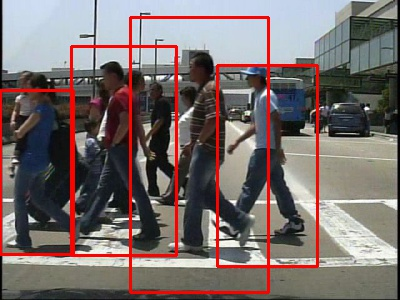
\includegraphics[width=7cm,height=5cm]{img/hog/1.jpg}}
\hspace{0.01\linewidth}
\subfigure[subfigure
 1-2]{\label{fig:subfig:b}
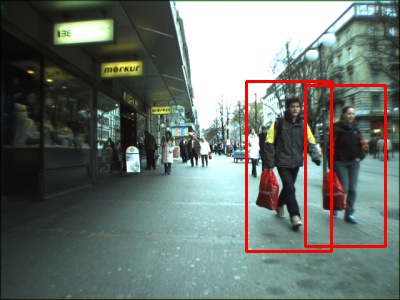
\includegraphics[width=7cm,height=5cm]{img/hog/2.jpg}}

\vfill

\subfigure[subfigure 2-1]{\label{fig:subfig:a}
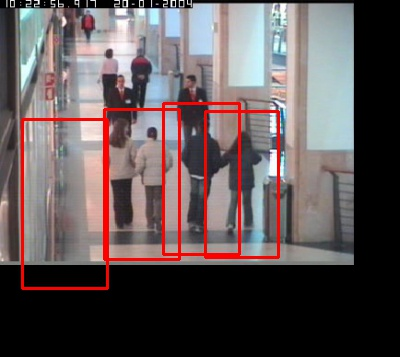
\includegraphics[width=7cm,height=5cm]{img/hog/3.jpg}}
\hspace{0.01\linewidth}
\subfigure[subfigure
 2-2]{\label{fig:subfig:b}
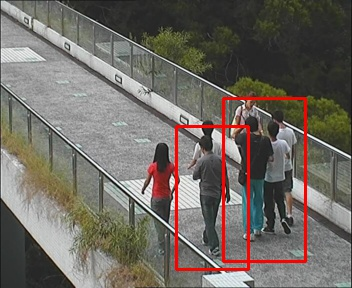
\includegraphics[width=7cm,height=5cm]{img/hog/4.jpg}}
\caption{HOG法检测行人}

\label{fig:hog}
\end{figure}

\subsubsection{Hog+SVM方法缺点}
可以看到,虽然Hog+SVM的方法可以成功的检测到行人,但是,直观看来,仍然存在着漏检,错检,以及检测框不够精准等诸多问题。且当输入图像变大的时候,滑窗数会急剧变多,算法速度直线下降。虽然,针对这一系列问题,学术界也有着相应的研究,但这不是本毕设的重点,也就不再赘述。本毕设将以此方法作为基准,在后续和各种深度学习检测结果进行比较。


\subsubsection{其他研究}
基于特征工程的方法研究行人检测,还有诸如SIFT特征,Haar特征,都取得了一定的突破,然而受限于低级特征的表达能力,这些方法的上限并不会太高。在深度学习大行其道的今天,如何利用深度学习解决这些问题,是学术界与工业界共同关心的问题,接下来的篇幅,将会着重介绍几种基于深度学习的行人检测算法。

\subsection{Faster-RCNN}
\subsubsection{算法概述}
Faster-RCNN是RCNN(Region Convolutional Nerual Network)算法的一种变体,RCNN经过了Fast-RCNN,Faster-RCNN的发展,以及最近更新的在像素层面上分割物体的Mask RCNN。
\par
\textbf{R-CNN:区域卷积神经网络}
这是基于卷积神经网络的物体检测的奠基之作。其核心思想是在对每张图片选取多个区域,然后每个区域作为一个样本进入一个卷积神经网络来抽取特征,最后使用分类器来对齐分类,和一个回归器来得到准确的边框。
整体流程如图所示\ref{fig:rcnn}

具体来说,这个算法有如下几个步骤:

\begin{itemize}
\item 对每张输入图片使用一个基于规则的“选择性搜索”算法来选取多个提议区域
\item 跟微调迁移学习里那样,选取一个预先训练好的卷积神经网络并去掉最后一个输入层。每个区域被调整成这个网络要求的输入大小并计算输出。这个输出将作为这个区域的特征。
\item 使用这些区域特征来训练多个SVM来做物体识别,每个SVM预测一个区域是不是包含某个物体
\item 使用这些区域特征来训练线性回归器将提议区域
\end{itemize}

\begin{figure}[htbp]
\begin{minipage}[t]{0.35\linewidth}
\centering
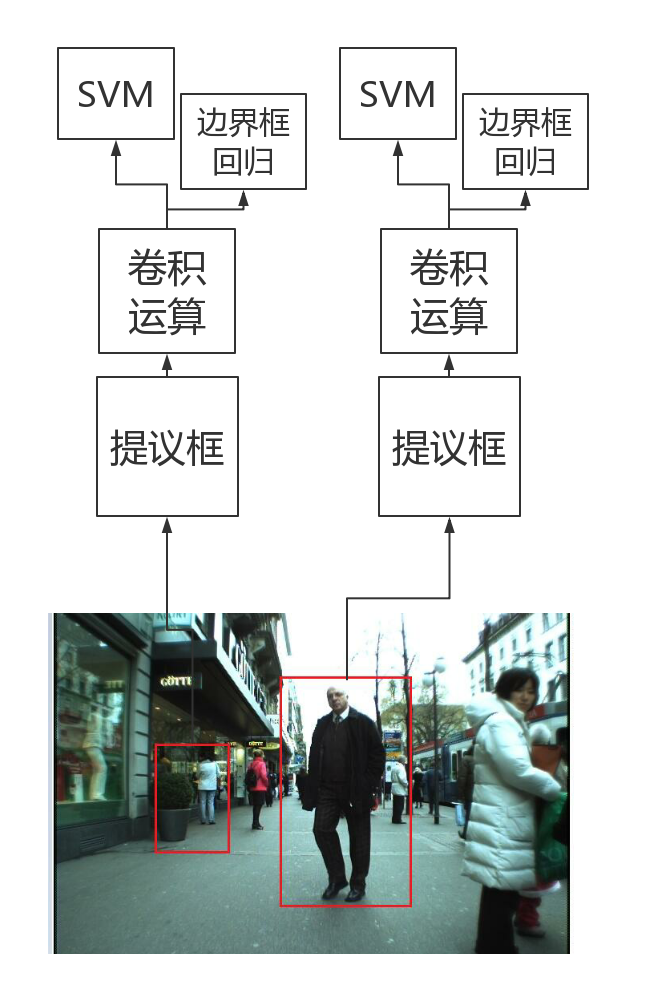
\includegraphics[height=8.5cm]{img/rcnn.png}
\caption{RCNN流程}
\label{fig:rcnn}
\end{minipage}%
\hfill
\begin{minipage}[t]{0.5\linewidth}
\centering
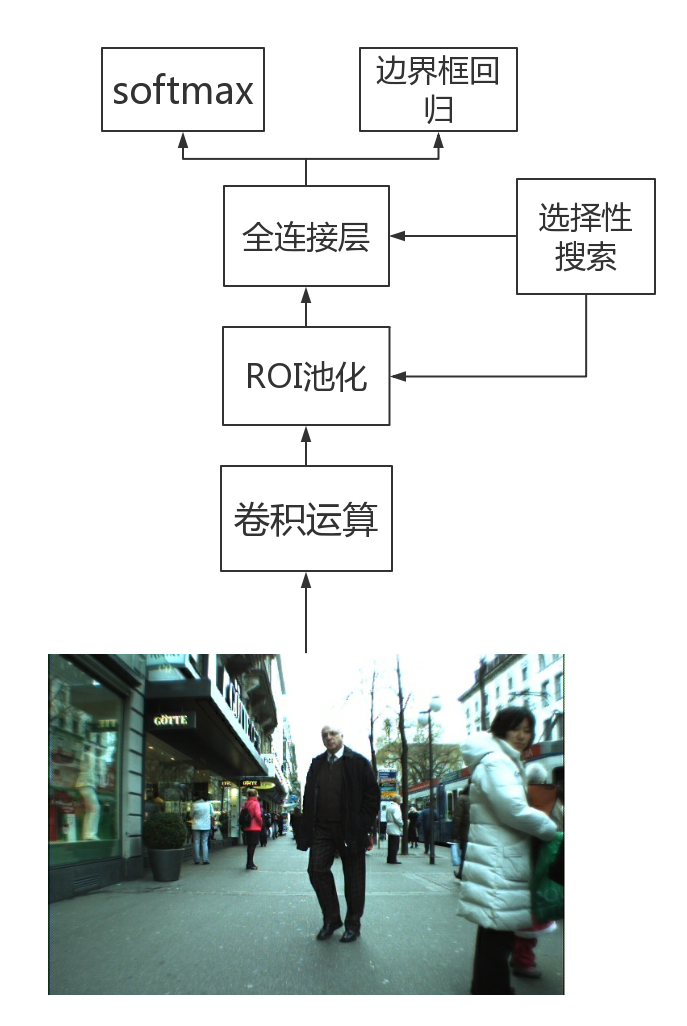
\includegraphics[height=8.5cm]{img/fast-rcnn.png}
\caption{Fast-RCNN流程}
\label{fig:fast-rcnn}
\end{minipage}
\end{figure}

直观上R-CNN很好理解,但问题是它可能特别慢。一张图片我们可能选出上千个区域,导致一张图片需要做上千次预测。虽然跟微调不一样,这里训练可以不用更新用来抽特征的卷积神经网络,从而我们可以事先算好每个区域的特征并保存。但对于预测,我们无法避免这个。从而导致R-CNN很难实际中被使用。

\textbf{Fast R-CNN:快速的区域卷积神经网络}
Fast R-CNN对R-CNN主要做了两点改进来提升性能。
\begin{itemize}
\item 考虑到R-CNN里面的大量区域可能是相互覆盖,每次重新抽取特征过于浪费。因此Fast R-CNN先对输入图片抽取特征,然后再选取区域。
\item Fast R-CNN不再使用多个SVM来做分类,而是用单个多类逻辑回归。
\end{itemize}

流程如图\ref{fig:fast-rcnn}所示

从示意图可以看到,使用选择性搜索选取的区域是作用在卷积神经网络提取的特征上。这样我们只需要对原始的输入图片做一次特征提取即可,如此节省了大量重复计算。
Fast R-CNN提出兴趣区域池化层(Region of Interest (RoI) pooling),它的输入为特征和一系列的区域,对每个区域它将其均匀划分成$n \times m$的小区域,并对每个小区域做最大池化,从而得到一个$n\times m$的输出。因此不管输入区域的大小,RoI池化层都将其池化成固定大小输出。

\textbf{Faster R-CNN:更快速的区域卷积神经网络}
Fast R-CNN沿用了R-CNN的选择性搜索方法来选择区域。这个通常很慢。Faster R-CNN做的主要改进是提出了区域提议网络(region proposal network, RPN)来替代选择性搜索。它是这么工作的:
\begin{itemize}
\item 在输入特征上放置一个padding为1,通道是256的$3\times 3$卷积。这样每个像素,连同它的周围8个像素,都被映射成一个长为256的向量。
\item 以每个像素为中心,生成$k$个大小和长宽比都预先设计好的默认边框,通常也叫锚框。
\item 对每个边框,使用其中心像素对应的256维向量作为特征,RPN训练一个2类分类器来判断这个区域是不是含有任何感兴趣的物体还是只是背景,和一个4维输出的回归器来预测一个更准确的边框。
\item 对于所有的锚框,个数为$nmk$如果输入大小是$n\times m$,选出被判断成还有物体的,然后前他们对应的回归器预测的边框作为输入放进接下来的RoI池化层
\end{itemize}

\begin{figure}[h]
\centering
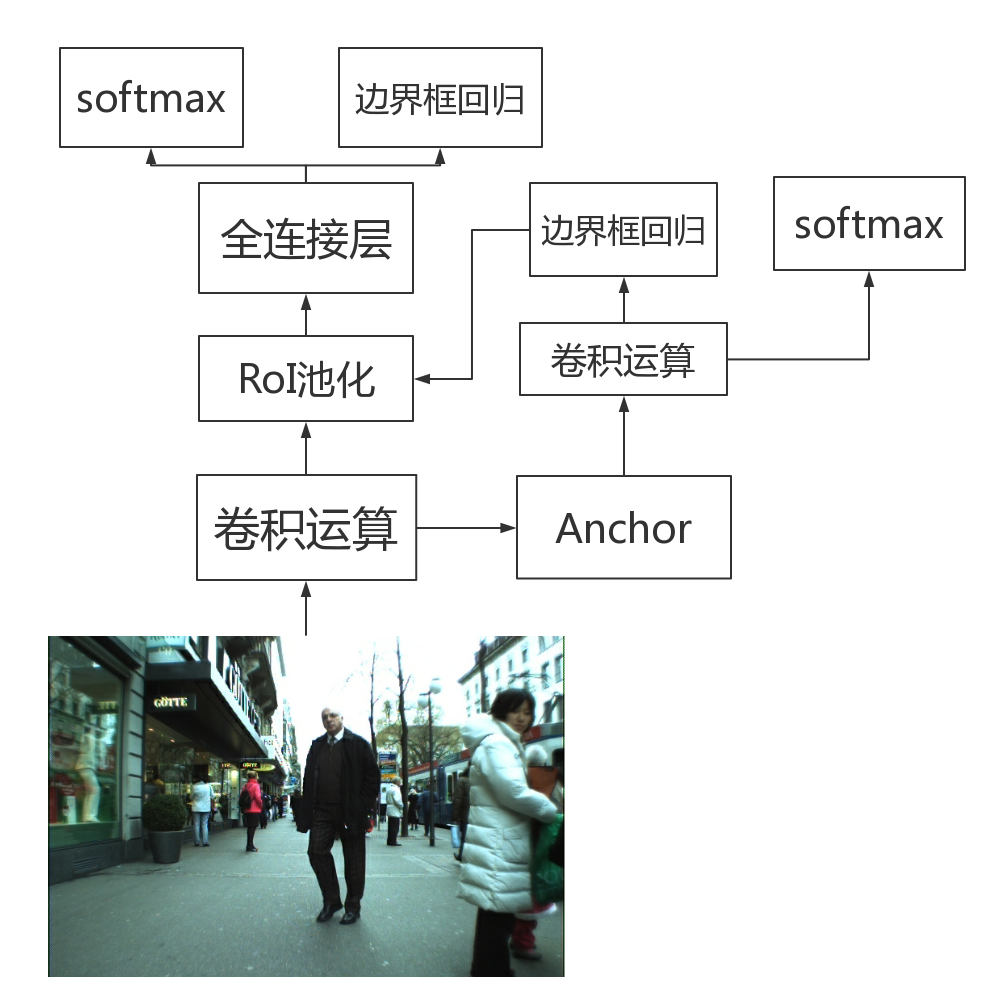
\includegraphics[height=8.5cm]{img/faster-rcnn.png}
\caption{Faster-RCNN流程}
\label{fig:faster-rcnn}
\end{figure}

虽然看上有些复杂,但RPN思想非常直观。首先提议预先配置好的一些区域,然后通过神经网络来判断这些区域是不是感兴趣的,如果是,那么再预测一个更加准确的边框。这样我们能有效降低搜索任何形状的边框的代价。\par
下面将分几节,介绍Faster-RCNN涉及的几个概念,其中,对于IoU和NMS在HoG的章节已经提及,可参考以上章节,将不再赘述。YOLO和SSD章节同理,相同概念不会重复介绍。

\subsubsection{特征抽取}
本章节所提及的所有Faster-RCNN结构,均默认是复用VGG16\upcite{simonyan2014very}网络的版本,下同,不特别注明。
对于一幅图像输入,Faster-RCNN首先对图像进行resize,然后通过一系列卷积组合运算得到一个feature map。而这个卷积运算,是复用分类网络(如VGG16)的feature extractor部分,这部分网络结构由13层卷积层,13层ReLU层,5层MaxPooling层组成。具体组合顺序和超参数,详见本毕设代码$fasterRCNN/lib/VGG16/faster\_rcnn\_vgg16.py$中的注释。ReLU层和MaxPooling层相关概念详见附录A。

\subsubsection{RPN}
RPN,Region Proposal Network,是Faster-RCNN相较于Fast-RCNN改进的点,用一个可整合进卷积网络的区域提议网络,代替之前的启发式的选择性搜索提出提议框。使整个算法模型成为一体式的网络结构,可统一用来训练和测试。RPN的结构图如\ref{fig:rpn}所示。

\begin{figure}[h]
\centering
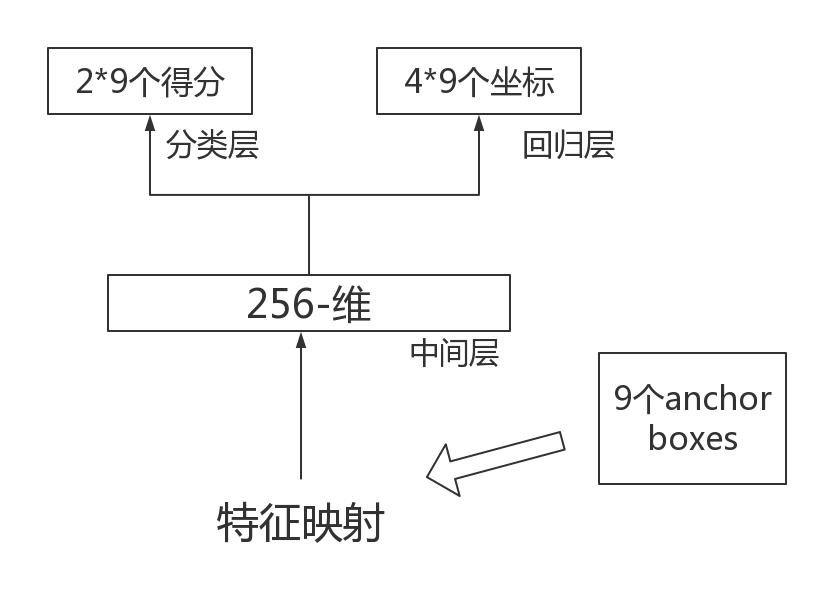
\includegraphics[height=5.5cm]{img/rpn.png}
\caption{RPN流程}
\label{fig:rpn}
\end{figure}
\par

其中,特征映射即上文提及的feature map,对于该feature map,用k个anchor boxes在该映射上的每一个点利用滑窗的思想,上下左右滑动,利用卷积计算中间层特征。在此之后,RPN分为两条支线,一侧得到该点上各anchor boxes对应的提议框的坐标x,y和长宽h,w,另一侧计算该点上各anchor boxes对应的提议框作为前景和背景的概率。TODO具体得到RoI

\textbf{anchor boxes:}
Anchor是大小和尺寸固定的候选框。默认的anchor由三种大小和三种长宽比,共9个。如图\ref{fig:anchorbox}。
\begin{figure}[h]
\centering
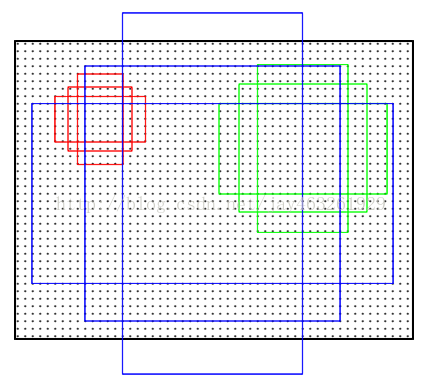
\includegraphics[height=5.5cm]{img/anchorbox.png}
\caption{Anchor示意图}
\label{fig:anchorbox}
\end{figure}

\textbf{训练损失函数:}回归的总Loss如公式\ref{eq:rpnLoss}:

\begin{equation}\label{eq:rpnLoss}
\begin{split}
& t_x = (x-x_a)/w_a,\quad t_y = (y-y_a)/h_a \\
& t_w = log(w/w_a),\quad t_h = log(h/h_a) \\
& t_x^* = (x^*-x_a)/w_a,\quad t_y^* = (y^*-y_a)/h_a\\
& t_w^* = log(w^*/w_a),\quad t_h^* = log(h^*/h_a) \\
& L({p_i},{t_i}) = \frac{1}{N_{cls}}\sum_iL_{cls}(p_i,p_i^*) + \lambda\frac{1}{N_{reg}}\sum_ip_i^*L_{reg}(t_i,t_i^*)
\end{split}
\end{equation}

其中,$x,y,w,h$为RPN网络预测的提议框的参数值,$x_a,y_a,w_a,h_a$为单一的anchor box对应的参数值,$x^*,y^*,w^*,h^*$为ground truth的框对应的参数值。

\subsubsection{RoI Pooling}
RoI Pooling本质上来说,可以理解成SPPnet\upcite{he2014spatial}的逆向。SPP-net对每个提议框使用不同尺寸的金字塔映射,而RoI pooling则是将RPN传进来的RoI区域对应的特征映射下采样到一个固定大小,比如$7\times 7$。而选择$7\times 7$的原因是因为当输入是$512\times7\times7$时候,将张量展开,将和VGG16的classfier的输入维度一致,后续可以继续复用预训练权重。通过RoI pooling的操作,可以将各种大小的所有提议框的原图特征映射下采样到固定大小的特征映射。将得到的特征映射张开成一维张量,送入复用的VGG16的两层全连接层。

\subsubsection{非极大值抑制}
与上文SVM+HoG算法中提到的非极大值抑制不同,Faster-RCNN整体流程中共用到了两次非极大值抑制。首先,在训练时,RPN网络中,第一次使用非极大值抑制,但这时候并没有考虑置信度,仅仅是依次排序,结果获得针对每个物体预测的第一个RoI。而之后,在预测阶段,就是同样地,对预测同一物体的预测框们,取置信度最高的作为最终的结果。

\subsubsection{Faster-RCNN整体流程}

\subsubsection{Faster-RCNN迁移到行人识别}
考虑到Faster-RCNN为多目标检测算法,它检测的目标数为数据

\subsubsection{实验表现}
PASCAL VOC 71.2 mAP   15FPS
\subsubsection{检测实例}
效果如图\ref{fig:rcnn}
\subsubsection{其他进展}
Faster RCNN的作者何恺明的Mask RCNN,以及专门针对检测人的论文\upcite{gkioxari2017detecting}。诸多实验室和人工智能公司都对Faster-RCNN有着复现,而2018年1月,Faster-RCNN作者所属机构Facebook的FAIR实验室正式开源了基于caffe2的detectron框架。这个框架有着一系列物体检测的接口,非常适合工程使用。

\begin{figure}[t]
\centering 
\subfigure[subfigure 1-1]{\label{fig:subfig:a}
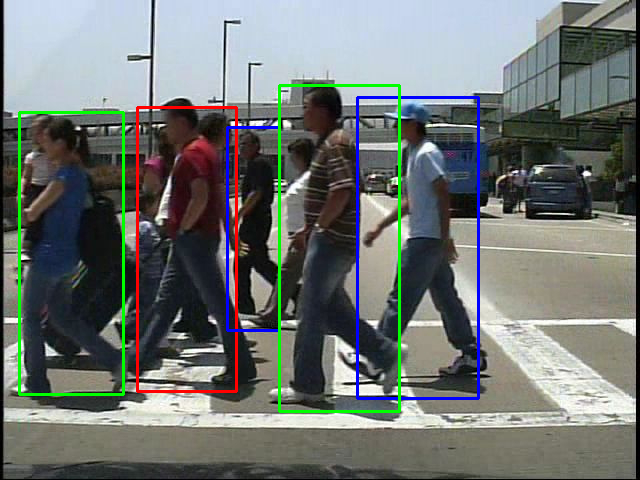
\includegraphics[width=7cm,height=5cm]{img/rcnn/1.png}}
\hspace{0.01\linewidth}
\subfigure[subfigure
 1-2]{\label{fig:subfig:b}
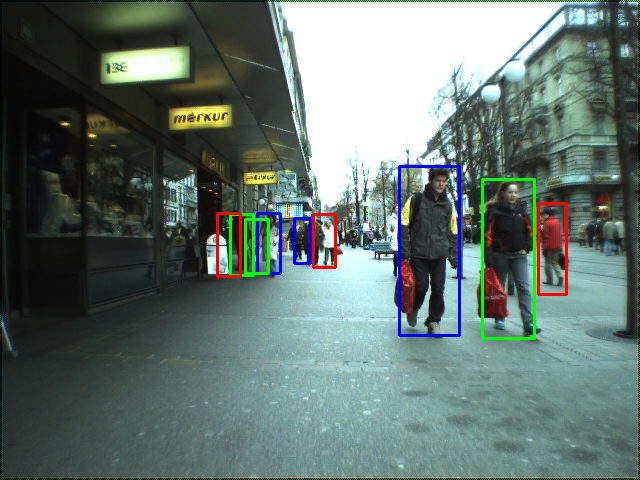
\includegraphics[width=7cm,height=5cm]{img/rcnn/2.png}}

\vfill

\subfigure[subfigure 2-1]{\label{fig:subfig:a}
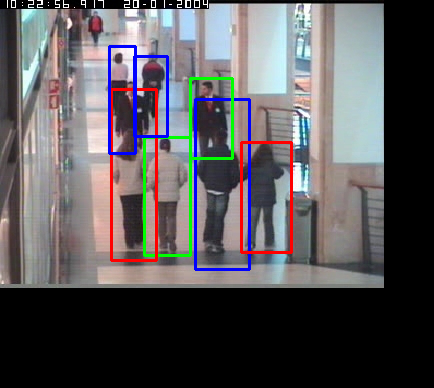
\includegraphics[width=7cm,height=5cm]{img/rcnn/3.png}}
\hspace{0.01\linewidth}
\subfigure[subfigure
 2-2]{\label{fig:subfig:b}
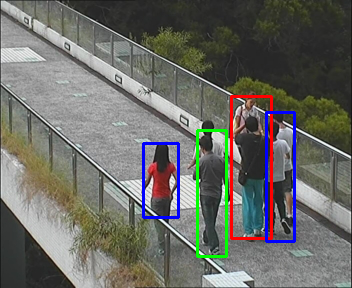
\includegraphics[width=7cm,height=5cm]{img/rcnn/4.png}}
\caption{Faster-RCNN法检测行人}

\label{fig:rcnn}
\end{figure}

\subsection{SSD}
\subsubsection{算法概述}
实际上,Faster RCNN在检测准确度和精度上已经达到了非常高的水平,但是它的检测速度实在是太慢了,难以满足实时的需求。SSD\upcite{liu2016ssd}(Single Shot MultiBox Detector)旨在平衡准确度和速度,相较于RCNN系列算法的先找提议框,再对提议框进行识别的“两步算法”不同,SSD算法试图将整个算法自图片输入到预测结果输出整合成一个整体流程。从而使整个模型简化且更加迅速。一般地,SSD首先复用一个物体识别网络,这里以VGG16为例,对于每一张输入图像,首先通过VGG16的feature extractor部分,之后原VGG16的全连接层被改写为卷积层接入其后,再连续通过4个作者定义的下采样卷积层。在这整个过程中,除了对于最终得到的特征输出外,还对其中5个不同阶段的中间特征图输出,采取边界框预测。预测则是通过在特征图的每一个点上应用default box预测多个边界框。最终将所有预测结果叠加,应用非极大值抑制得到最终的输出。值得一提的是,SSD自始至终都只用了卷积运算,所以它是全卷积网络(Fully Convolutional Network),由于卷积操作并不受输入层的大小的限制,所以它对输入图像大小不敏感,对于任意大小的输入图像都能正常运作。
\subsubsection{default box}
SSD所使用的default box和Faster RCNN部分使用的anchor box非常类似,都是由不同大小和长宽比组成的包围盒,应用在特征图的每一个点上,但两者有以下区别:
\begin{itemize}
\item Faster RCNN只在最终的输出特征图上应用一个anchor box。而SSD则在包括最终输出和中间输出的特征图上多次使用了default box。
\item 对于anchor box,m个aspect和n个scale会生成,$m\times n$个包围盒,但对于default box只会生成$m+n-1$个包围盒。
\end{itemize}

具体来说,对于给定的特征图的每一个点,SSD在其中心以不同大小和长宽比的边界框进行采样,假定输入的大小是$w \times h$。
\begin{itemize}
\item 给定大小 $s\in (0,1]$,那么生成的边界框形状是 $ws \times hs$
\item 给定长宽比 $r > 0$,那么生成的边界框形状是 $w\sqrt{r} \times \dfrac{h}{\sqrt{r}}$
\end {itemize}

default box如图\ref{fig:defaultBox}所示

\begin{figure}[h]
\centering
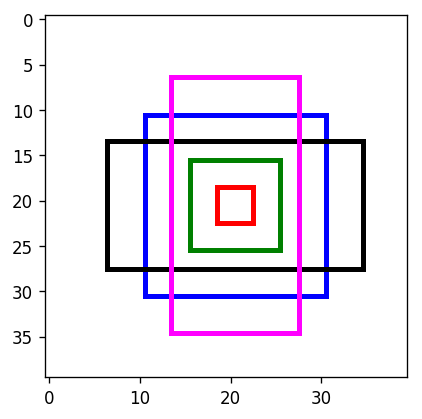
\includegraphics[height=5.5cm]{img/defaultBox.png}
\caption{default box示意图}
\label{fig:defaultBox}
\end{figure}

另外,对于不同阶段的特征图,default box采用了不同大小以更好的拟合边界框:高维度的特征图有着较大的包围盒尺寸。

\subsubsection{1 $\times$ 1的卷积}
SSD运算过程中,多次使用了$1 \times 1$的卷积,这种卷积由Network in Network\upcite{lin2013network}论文首次提出,并由GoogLeNet\upcite{szegedy2015going}的应用而获得广泛推广。

$1\times 1$卷积的作用可以理解为对输入层的每个点应用一个全连接层。具体的步骤是,对于输入层,该卷积算子遍历输入值信道(channel)的每一个值,并加权累加它们,输出到一个ReLU层进行非线性转换。而输出特征图的信道数等于卷积算子的数量(\#filter)。\par

应用这种算子最主要的原因是可以极大的减少运算量。以VGG16版本输入图像大小为300的SSD举例。Conv7大小为$19 \times 19 \times 1024$依次应用$1 \times 1 \times 256$和$3 \times 3 \times 512 stride = 2$的卷积得到大小为$10 \times 10 \times 512$的输出Con8\_2。
\begin{itemize}
\item 在不使用$1 \times 1$卷积的情况下,参数量为$10 \times 10\times 512\times 3 \times 3 \times 1024 /2 \approx2.36$亿
\item 在使用$1 \times 1$卷积的时候,参数为分两部分,第一部分是从输入层Conv7经过$1\times 1$卷积的中间输出,为$19\times 19\times 256\times 1024\approx 0.59$亿。第二部分由中间输出到Con8\_2,参数量为$10\times 10\times 512\times 3\times 3\times 256/2 \approx0.95$亿,共为$1.54$亿
\end{itemize}

综上,在使用了$1\times 1$的卷积后,参数减少了约35\%。这对追求效率的算法而言,是个非常有益的。因此这样的卷积也常常被称之为瓶颈(bottlenect)。同时大量的实验证明,对于瓶颈选用合适的信道数是可以保证性能不下降的。

\subsubsection{检测实例}

如图\ref{fig:ssdDetect}

\begin{figure}[t]
\centering 
\subfigure[subfigure 1-1]{\label{fig:subfig:a}
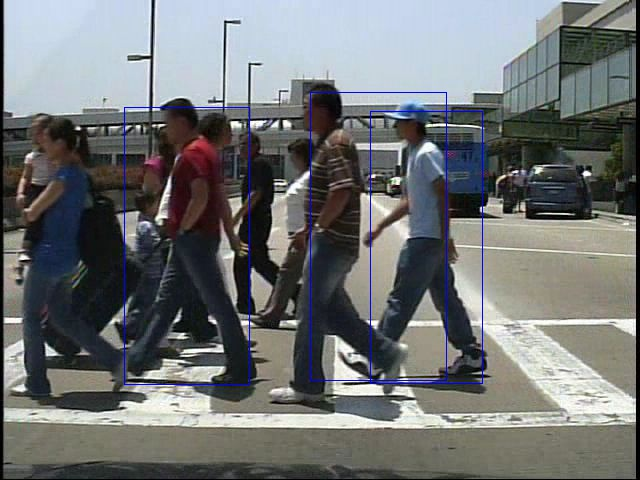
\includegraphics[width=7cm,height=5cm]{img/ssd/1.jpg}}
\hspace{0.01\linewidth}
\subfigure[subfigure
 1-2]{\label{fig:subfig:b}
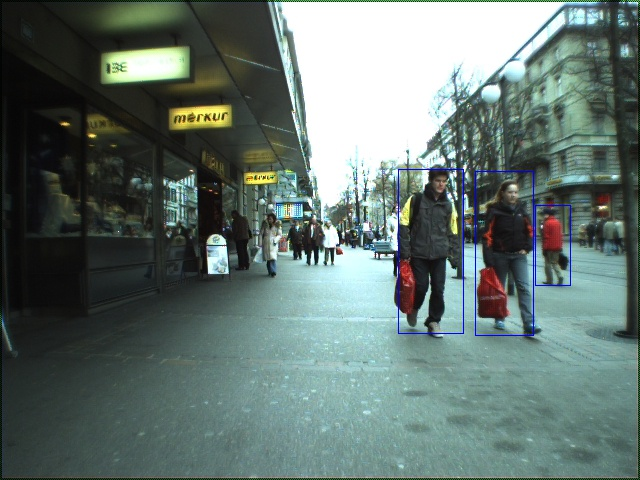
\includegraphics[width=7cm,height=5cm]{img/ssd/2.jpg}}

\vfill

\subfigure[subfigure 2-1]{\label{fig:subfig:a}
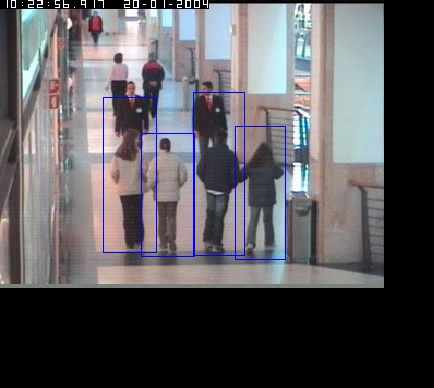
\includegraphics[width=7cm,height=5cm]{img/ssd/3.jpg}}
\hspace{0.01\linewidth}
\subfigure[subfigure
 2-2]{\label{fig:subfig:b}
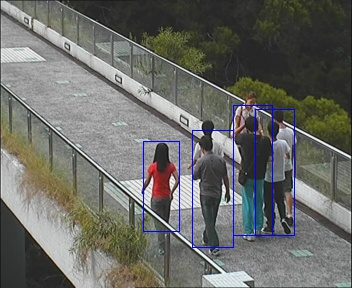
\includegraphics[width=7cm,height=5cm]{img/ssd/4.jpg}}
\caption{SSD300检测行人}

\label{fig:ssdDetect}
\end{figure}


\subsubsection{算法性能提升}
1. 高分辨率  512
2. 更好的特征提取网络 ResNet

\subsubsection{其他进展}
DSSD


\subsection{YOLO}
\subsubsection{算法概述}
YOLO(You only look once),自发布至今已迭代更新三个版本。v1\upcite{redmon2016you},v2\upcite{redmon2017yolo9000},v3\upcite{}。\par
\textbf{YOLOv1} 不同于Faster-RCNN等two-stage算法,YOLO和SSD一样,将整个算法流程整合成了一个回归问题,故它是one-stage算法。整个网络由24个卷积层和2个全连接层组成。最终输出结果为一个S$\times S \times(5\times B + C)$的张量,S表示输出特征图的大小,典型值为7,B代表特征图的每个cell上预测的边界框的数量,典型值为2,C为总共需要预测的数量,论文训练使用的是PASCAL VOC数据集,所以C=20。对于输出特征图的每一个cell点,有它预测的两个边界框的中心坐标和长宽,以及它作为准确边界框的置信度。剩下的20个值分别为每个类别的概率。通过这样的设计,训练得到的模型,可以直接从输入图像得到检测结果,速度非常的快。YOLOv1在相对准确的前提下,速度大幅度提高。但YOLOv1的缺点也非常明显,由于他对于特征图输出的每个cell只预测两个边界框,且同类型的物体中心落到同一个cell的话,只会预测其中一个,这直接导致了YOLOv1对于同物体密集型的场景适用性很差,比如交通行人检测。同时,YOLOv1的边界框是相对输入图像大小的,从而很难学习不同长宽比的物体,这也使得他的定位准确度较差。且YOLOv1的特征图大小是单一的,为$7\times 7$,这使得他对于颗粒度小的物体并不敏感。同时,由于最后的分类层是传统的全连接层,这导致YOLOv1的参数非常的多,且要求输入图像大小固定。\par
\textbf{YOLOv2}  YOLOv2在YOLOv1的模型基础上,增加了多种尝试,使得在维持高检测速度的前提下,大幅提高准确度。引入Batch Normalization\upcite{ioffe2015batch}机制,使用高分辨率图像如$448 \times 448$,从而获得更多特征,使用anchor boxes机制,边界框聚类技术最终大幅提高了检测准确度和定位精度。\par
\textbf{YOLOv3}  相较于YOLOv2,最新版本的YOLO使用了多尺度预测的方法,聚类边界框等技巧提高准确度,以及相较于YOLOv2的darknet-19更深的特征提取网络,该网络里增添了ResNet\upcite{he2016deep}的skip connection机制。最终YOLOv3的对比如图\ref{fig:yoloPerform}

\begin{figure}[h]
\centering
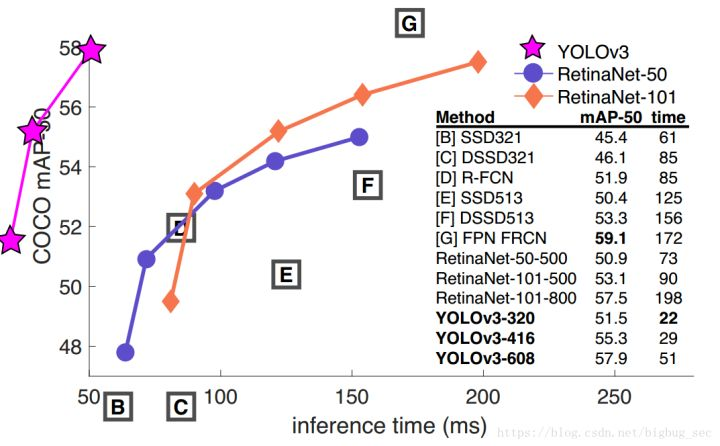
\includegraphics[height=6.5cm]{img/yolov3.jpg}
\caption{yolov3表现}
\label{fig:yoloPerform}
\end{figure}

\subsubsection{batch normalization}
假定神经网络一层的输出为$z^{(1)}, z^{(2)}, .... , z^{(m)}$,对它们做如下代换:

\begin{align}
 &\mu = \frac{1}{m}\sum_iz^{(i)} \\
 &\sigma = \frac{1}{m}\sum_i(z^{(i)}-\mu)^2 \\
 &z^{(i)}_{norm} = \frac{z^{(i)}-\mu}{\sqrt{\sigma^2+\varepsilon}}
\end{align}

如此,使得所有分量满足均值为0,方差为1的分布。进一步地,为了能够更好的拟合,可以继续做如下变换:

\begin{equation}
\widetilde{z}^{(i)} = \gamma z_{norm}^{(i)}+\beta
\end{equation}
其中,$\gamma$和$\beta$都是可以学习更新的参数。\par
Batch Norm使得每次梯度下降都能够更加的趋近最值点,也避免了隐藏层的激活值进入饱和阶段,使得每一层的值能够更好的传递下去,加速模型训练速度,更是避免了梯度弥散的情况。

\subsubsection{Skip Connection}
传统卷积神经网络,往往通过增加卷积层加深网络深度,从而提取更加高维的特征,提升性能,但这么做会导致一个严重的问题--梯度弥散/消失(Vanishing),在反向传播的过程中,梯度会随着传播的进行快速下降,随着网络加深,梯度弥散会愈发严重,直接导致网络的前部分权重无法充分的训练。而在ResNet中提出的skip connection机制能够有效解决这个问题。我们一段多层卷积层(称之为块)旁边增加一条捷径,假定块的输入为x,该块的输出为f(x),块的输出和捷径相加得到的最终输出值f(x)+x。这样,在反向传播的过程中,会多一项dx//dx的输出,也即梯度为1,如此,深层的梯度能够更完整的传递,使得浅层网络得到充分的训练。

\subsubsection{多尺度预测}
不同于之前的YOLO版本,最新版本的YOLO不再是仅仅生成一个特征图输出(典型值为7),而是同时对输入图像生成3个不同大小的输出特征图,输入图像大小为$416\times 416$的时候,典型值分别为13, 26, 52。这样,一幅图像,我们的算法将预测$((52\times 52)+(26\times 26)+(13\times 13))\times 3$个边界框,后面的系数3是对于特征图输出的每个cell预测3个边界框。这么做有效的减少了YOLO之前存在的对于小颗粒度物体检测准度不高的缺陷。考虑到这么做同时会加重网络预测的开销,YOLOv3同时采取了置信度阈值机制和最大值抑制的方法:当某边界框的置信度低于设定的阈值的时候,算法会过滤掉这些边界框。而最大值抑制,则主要为了避免同一物体的多次检测,详情请参考本毕设先前部分。

\begin{figure}[h]
\centering
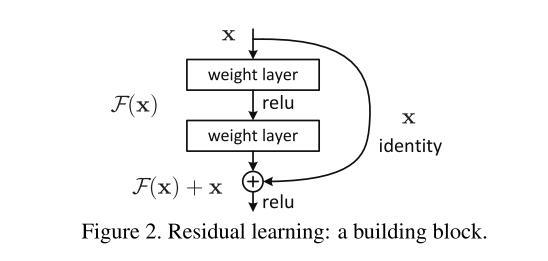
\includegraphics[height=4.5cm]{img/shortcut.jpg}
\caption{shortcut}
\label{fig:shortcut}
\end{figure}

\subsubsection{YOLO检测流程}
\textbf{YOLO}:  YOLOv1实际上的流程非常简单,如图\ref{}, 所示
\textbf{YOLOv3}:虽然YOLOv3是全卷积网络,也就是对输入图像的大小并不敏感,但是考虑到实际应用的时候,我们常常会设定Batch Size大于1用以提升速度,为此将输入图像大小固定会有利于我们实现算法。且考虑到YOLOv3会在步幅分别为8,16,32的三个不同规模下进行,所以我们固定resize图像为416。接下来送入算法定义的特征提取网络,因为一共有53层,作者命其为darknet-53,如图\ref{fig:darknet53}。这部分将输出$((52\times 52)+(26\times 26)+(13\times 13))\times 3$个边界框,每个边界框有$(5+C)$个值,其中5表示为中心坐标($x_{center}, y_{center}$),长宽值($w, h$)和物体置信度。C表示的为数据集的类别数,原论文使用的是COCO\upcite{}数据集,该值为80。进一步地,由于每一个检测框仅仅只会表示一个单一类,所以对于这些所有的边界框,我们对它们只保留C个值中最大的类别。同时,同之前所提的,对于物体置信度低于阈值的边界框项,将直接无视。对于那些置信度大于阈值的所有边界框,进行非极大值抑制的操作,依次计算两两预测框之间的交并比值,若高于设定的iou阈值,则只保留该类别得分更高的那项,重复直至不存在高于iou阈值的两个预测框。

\begin{figure}[h]
\centering
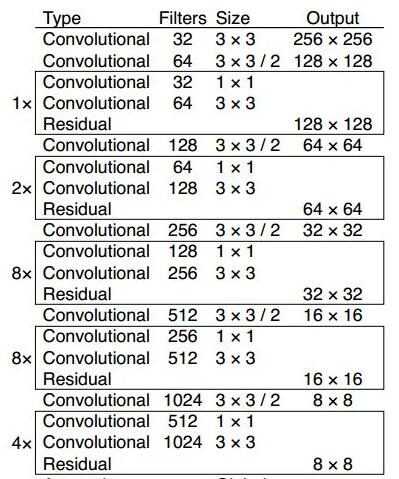
\includegraphics[height=8.5cm]{img/darknet53.jpg}
\caption{shortcut}
\label{fig:darknet53}
\end{figure}


\subsubsection{实验表现}
PACAL VOC 63.0 mAP    45FPS
\subsubsection{检测实例}
效果如图\ref{fig:yolov3}所示。直观上看,最新版的YOLO具有比之前提到的算法都更好的识别准确度和定位精度。

\subsubsection{实现细节}
1. 坐标变换
2. 

\begin{figure}[t]
\centering 
\subfigure[subfigure 1-1]{\label{fig:subfig:a}
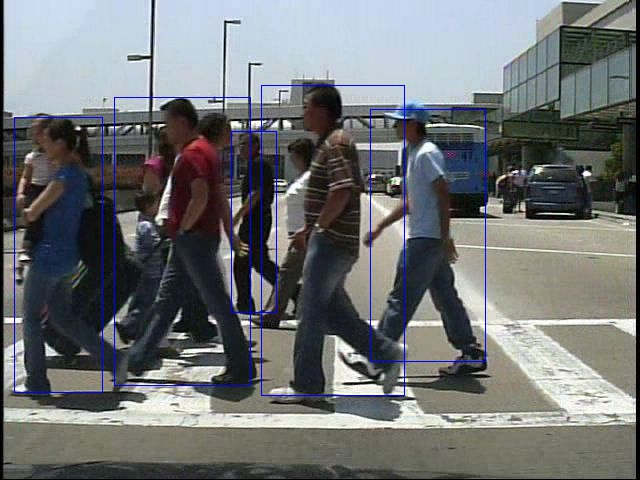
\includegraphics[width=7cm,height=5cm]{img/yolo/1.jpg}}
\hspace{0.01\linewidth}
\subfigure[subfigure
 1-2]{\label{fig:subfig:b}
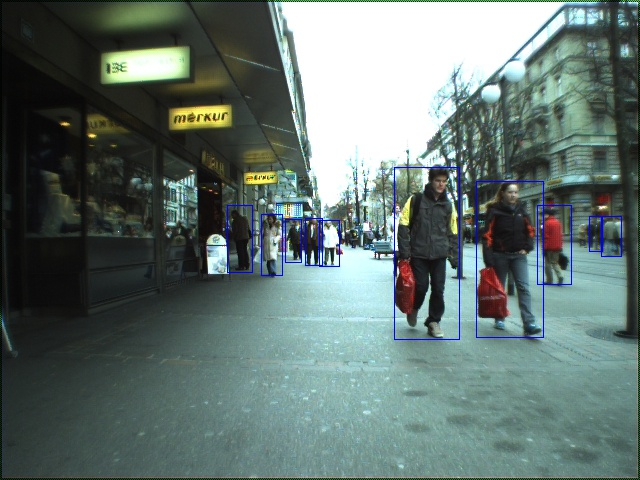
\includegraphics[width=7cm,height=5cm]{img/yolo/2.jpg}}

\vfill

\subfigure[subfigure 2-1]{\label{fig:subfig:a}
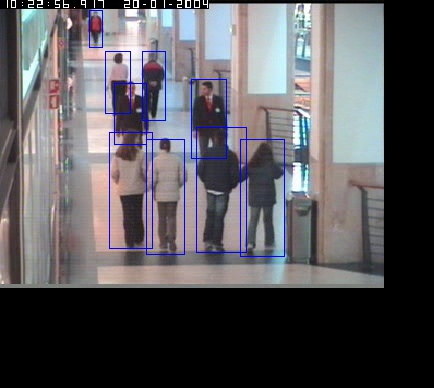
\includegraphics[width=7cm,height=5cm]{img/yolo/3.jpg}}
\hspace{0.01\linewidth}
\subfigure[subfigure
 2-2]{\label{fig:subfig:b}
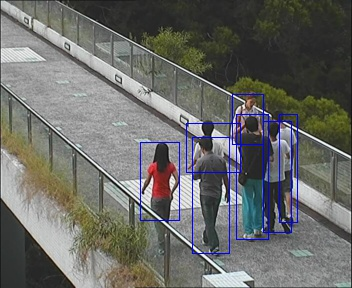
\includegraphics[width=7cm,height=5cm]{img/yolo/4.jpg}}
\caption{YOLOv3检测行人}

\label{fig:yolov3}
\end{figure}

\section{迁移学习尝试}
考虑到SSD在中间层多次使用预测,Faster RCNN结构复杂,上述三种算法最适合应用微调策略是YOLO。
1. 对于网络仅仅修改特征提取的最后一层,使得能够快速的在小数据集上迭代出结果
2. 迁移学习目前存在的问题:遮挡过多无法检测,夜景,


\section{算法的实际场景应用}
通过迁移学习的方法,在充分训练的前提下,这些目标检测算法可以非常适合的迁移到诸如人脸检测,交通信号牌检测等等其他问题上去。

\section{一些失败的尝试}


\section*{致谢}
\addcontentsline{toc}{section}{致谢}


\newpage
\renewcommand\refname{\zihao{-2} 参考文献}
\addcontentsline{toc}{section}{参考文献}
\bibliographystyle{plain}     %按引用顺序
\bibliography{bio}

\newpage
\section*{附录A}
\addcontentsline{toc}{section}{附录A}

\subsection*{涉及概念的关系}


\subsection*{神经网络}
\subsubsection*{神经网络简介}

常见的神经网络结构是如图\ref{fig:nn}所示的层级结构。
\begin{figure}[htbp]
\begin{minipage}[t]{0.35\linewidth}
\centering
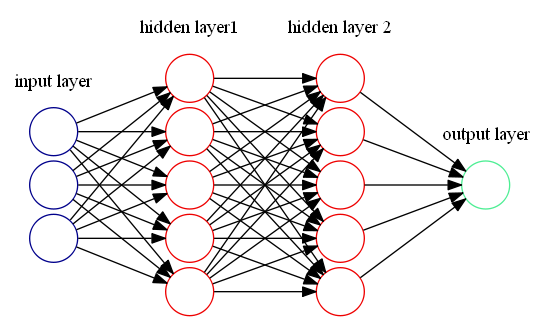
\includegraphics[height=4.5cm]{img/neural_network.png}
\caption{双隐层前馈网络}
\label{fig:nn}
\end{minipage}%
\hfill
\begin{minipage}[t]{0.5\linewidth}
\centering
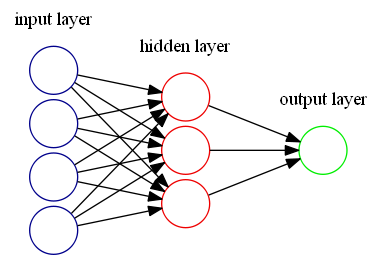
\includegraphics[height=4.5cm]{img/nn431.png}
\caption{4结点输入单隐藏层网络}
\label{fig:sample}
\end{minipage}
\end{figure}
图中,每个结点代表一个神经元,神经元是神经网络构成的最基本成分,当神经元的接收到的总输入值超过了阈值,则该神经元通过激活函数(activation function)对后续神经元产生输出。输入层与输出层之间的每层神经元,被称为隐层或者隐含层(hidden layer),隐含层和输出层的神经元都是拥有激活函数的功能神经元。每层神经元与下一层神经元全互联,神经元之间不存在同层连接,也不存在跨层连接。这样的神经网络结构通常称为“多层前馈神经网络”(multi-layer feedforward neural networks)。图示即为双隐层前馈网络。输入层神经元接受外界输入,隐层与输出层神经元对信号进行加工,最终结果由输出层神经元输出。神经网络的学习过程,就是根据训练数据来调整神经元之间的“连接权”(connection weight)以及每个功能神经元的阈值。\par
\subsubsection*{神经网络在计算机视觉上的应用}
以图像识别任务为例,假设一个图像是大小$2 \times 2$的灰度图像,那么在将它在计算机上将以一个$1 \times 2 \times 2$的矩阵储存,在送入神经网络进行分类之前,需要将其展开成一维向量。此时网络的输入结点是4,假定网络隐藏层个数为3,仅一层,且为二分类问题,则网络如图\ref{fig:sample}所示。
第一层到第二层有$4 \times 3 = 12$个参数,第二层有$3\times 1 = 3 $个参数。共计15个权重(weights)参数。\par
神经网络曾引起一阵效仿的热潮,但其收敛缺乏理论证明,性能也渐渐被其他分类器超越。神经网络主要主要存在以下缺点:
\begin{itemize}

   \item 未考虑空间因素。
   \item 输入图像较大,或网络层数,结点数较大时,参数巨大。
\end{itemize}

\subsubsection*{前向传播和反向传播}

所以渐渐的
\subsection*{卷积网络}
卷积网络(convolutional network)(LeCun,1989),也叫做卷积神经网络(convolutional nerual ntework, CNN),是一种专门用来处理具有类似网格结构的数据的神经网络。例如时间序列数据(可以认为是在时间轴上有规律地采样形成的一维网格)和图像数据(可以看做二维的像素网格)。卷积网络在诸多应用领域都表现优异。“卷积神经网络”一词表明该网络使用了卷积(convolution)这种数学运算。卷积是一种特殊的线性运算。卷积网络是指那些至少在网络的一层中使用卷积运算来代替一般的矩阵乘法运算的神经网络。
\paragraph{卷积运算}
值得注意的是,深度学习中所指的卷积,和一般工程领域或数学领域的卷积运算并不相同。在通常形式中,卷积是对两个实变函数的一种数学运算。
\[
s(t)=\int x(a)w(t-a)da
\]
这种运算就叫做卷积。卷积常用星号表示:
\[
s(t) = (x*w)(t)
\]
在卷积网络的术语中,卷积的第一个参数(参数x)通常叫做输入(input),第二个参数(函数w)叫做核函数(kernel function)。输出有时被称作特征映射(feature map)。如果时刻t只能取整数值。且假定x和w都定义在整数时刻t上,就可以定义离散形式的卷积:
\[
s(t) = (x*w)(t) = \sum_{a=-\infty}^{\infty}x(a)w(t-a)
\]
在机器学习应用中,输入通常是多维数组的数据,而核通常是由学习算法优化得到的多维数组的参数。我们把这些多维数组叫做张量。因为在输入与核中的每一个元素都必须明确地分开存储,我们假定在存储了数值的有限点集以外,这些函数的值都为0。这意味着在实际操作中,我们可以通过对有限个数组元素的求和来实现无限求和。最后,我们通常一次在多个维度上进行卷积运算。例如一张二维图像作为输入,我们也许也想要使用一个二维的核K:
\[
S(i,j) = (I*K)(i,j) = \sum_m\sum_nI(m,n)K(i-m,j-n)
\]
许多神经网络库会实现一个相关的函数,称为互相关函数(cross-correlation),和卷积运算几乎一样但是并没有对核进行翻转。
\[
S(i,j) = (I*K)(i,j) = \sum_m\sum_nI(i+m,j+n)K(m,n)
\]
许多机器学习库实现的是互相关函数但是称之为卷积。

通俗来说,核(过滤器)在输入数据(张量)上依次滑动,通过卷积(互相关)运算,得到输出(特征映射)。
图\ref{fig:conv}演示了一个在二维张量上的卷积运算例子。
\begin{figure}[ht]

\centering
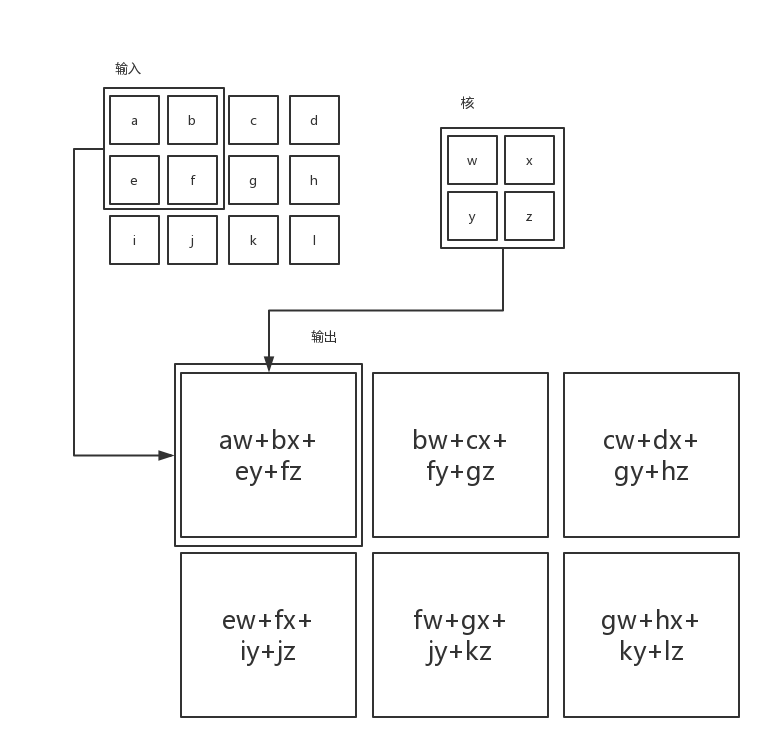
\includegraphics[height=8.5cm]{img/convolution.png}
\caption{一个二维卷积的例子}
\label{fig:conv}
\end{figure}

\paragraph{动机}
卷积运算通过三个重要的思想来帮助改进机器学习系统:稀疏交互(sparse interactions)、参数共享(parameter sharing)、等变表示(equivariant representations)。另外,卷积网络还提供了一种处理大小可变的输入的方法。\par
传统神经网络使用矩阵乘法来建立输入与输出的连接关系。其中,参数矩阵中每一个单独的参数都描述了一个输入单元与一个输出单元间的交互。这意味着每一个输出单元与每一个输入单元都产生交互。然而,卷积网络具有稀疏交互(sparse interactions(也叫做稀疏连接(sparse connectivity)或者稀疏权重(sparse weights))的特征。这是使核的大小远小于输入的大小达到的。举个例子,当处理一张图像时,输入的图像可能包含成千上万个像素点,但是我们可以通过只占用几十到上百个像素点的核来检测一些小的有意义的特征,例如图像的边缘。这意味着为了得到输出我们只需要更少的计算量。这些效率上的提高是很显著的。如果有$m$个输入和$n$个输出,那么矩阵乘法需要$m \times n$个参数并且相应算法的复杂度为$O(m \times n)$(对于每一个例子)。如果我们限制每一个输出拥有的连接数为$k$,那么稀疏的连接方法只需要$k \times n$个参数以及$O(k\times n)$的运行时间。在很多实际应用中,只需要保持$k$比$m$小几个数量级,就能在机器学习的任务中取得好的表现。稀疏连接的图形化解释如图\ref{fig:sparse_dense} 和图\ref{fig:sparse_dense_receptive_field}。在深度卷积网络中,处在网络深层的单元可能与绝大部分输入是间接交互的,如图\ref{fig:receptive_field}。这允许网络可以通过只描述稀疏交互的基石来高效地描述多个变量的复杂交互。

\begin{figure}[htbp] %子图上下居中对齐

\centering

\subfigure[]{
\begin{minipage}[c]{0.5\textwidth}
\centering
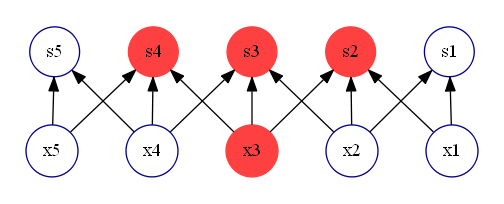
\includegraphics[width=8.5cm]{img/sparse_connect.png}
\end{minipage}
}


\subfigure[]{
\begin{minipage}[c]{0.5\textwidth}
\centering
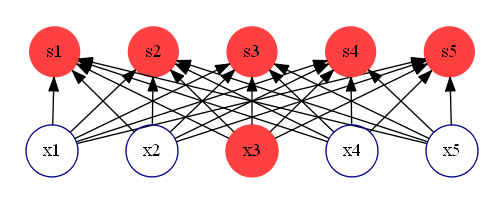
\includegraphics[width=8.5cm]{img/dense_connect.png}
\end{minipage}
}

\caption{稀疏连接,对每幅图从下往上看。我们强调了一个输入单元$x_3$以及在$s$中受该单元影响的输出单元。(a)当$s$是由核宽度为3的卷积产生时,只有三个输出受到$x$的影响。(b)当s是由矩阵乘法产生时,连接不再是稀疏的,所以所有的输出都受到$x_3$的影响}
\label{fig:sparse_dense}
\end{figure}

\begin{figure}[htbp] %子图上下居中对齐
\centering

\subfigure[]{
\begin{minipage}[c]{0.5\textwidth}
\centering
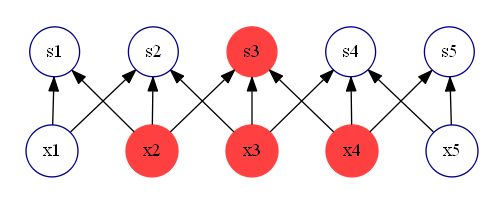
\includegraphics[width=8.5cm]{img/sparse_receptive_field.png}
\end{minipage}
}


\subfigure[]{
\begin{minipage}[c]{0.5\textwidth}
\centering
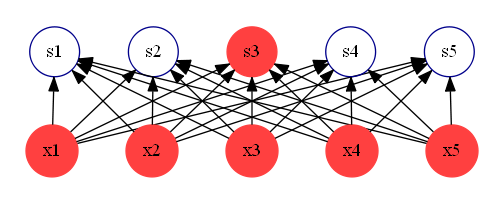
\includegraphics[width=8.5cm]{img/dense_receptive_field.png}
\end{minipage}
}

\caption{稀疏连接,对每幅图从下往上看。我们强调了一个输入单元$x_3$以及在$x$中影响该单元的输入单元。这些单元被称为$s_3$的接受域(receptive field)。(a)当$s$是由核宽度为3的卷积产生时,只有3个输入影响$s$。(b)当$s$是由矩阵乘法产生时,连接不再是稀疏的,所以所有的输入都会影响$s_3$}
\label{fig:sparse_dense_receptive_field}
\end{figure}

\par
参数共享(parameter sharing)是指在一个模型的多个函数中使用相同的参数。在传统的神经网络中,当计算一层的输出时,权重矩阵的每一个元素只使用一次,当它乘以输入的一个元素后就再也不会用到了。作为参数共享的同义词,我们可以说一个网络含有绑定的权重(tied weights),因为用于一个输入的权重也会被绑定在其他的权重上。在卷积神经网络中,核的每一个元素都作用在输入的每一位置上(是否考虑边界像素取决于对边界决策的设计)。 卷积运算中的参数共享保证了我么只需要学习一个参数集合,而不是对于每一位置都需要学习一个单独的参数集合。这虽然没有改变前向传播的运行时间(仍然是$O(k\times n)$),但它显著地把模型的存储需求降低至$k$个参数,并且$k$通常要比$m$小很多个数量级。因为$m$和$n$通常有着大致相同的大小,$k$在实际中相对于$m \times n$是很小的。因此,卷积在存储需求和统计效率方面极大地优于稠密矩阵的乘法运算。

\paragraph{激活函数}
神经网络最终还是一个非线性模型,而上述的层与层的连接都是线性的,可以证明的是,无论神经网络多少层,只要全是线性的,就总可以等价成一种单层的线性表达。基于此,我们需要在神经网络中加入非线性因素。一个惯用的做法是,在每层网络层的输出位置,加上一个激活函数,也即当网络层的输出值大于激活函数的阈值时,这一层的输出才传往下一层,否则置零。常见的激活函数有tanh函数,和ReLU函数

\paragraph{ReLU}
Rectified Linear Unit,线性修正单元。考虑到tanh作为激活函数时,有着梯度消失的风险。经过研究人员的不断尝试,于AlexNet(存疑,待确认)首次提出了ReLU,ReLU本质是一个分段函数,

\paragraph{池化层}
Maxpooling



\begin{figure}[htbp]

\centering
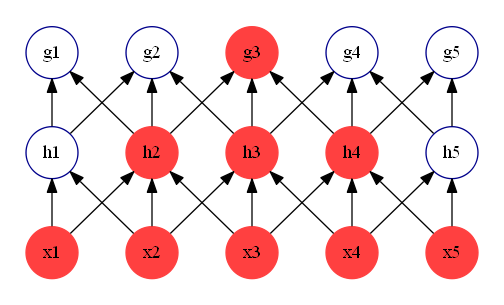
\includegraphics[width=8.5cm]{img/deep_receptive_field.png}
\caption{处于卷积网络更深的层中的单元,它们的接受域要比处在浅层的单元的接受域更大。如果网络还包含类似步幅卷积或者池化之类的结构特征,这种效应会加强。这意味着在卷积网络中尽管直接连接都是很稀疏的,但处在更深的层中的单元可以间接地连接到全部或者大部分输入图像}
\label{fig:receptive_field}
\end{figure}

\newpage
\section*{附录B}
\addcontentsline{toc}{section}{附录B}

\section*{翻译}

\subsection*{Faster-RCNN}

\paragraph {摘要:}
最先进的目标识别网络决定于区域推荐算法去假设目标所在。先进的如SPPnet和Fast R-CNN降低了这些检测网络的运行时间,同时暴露出区域提出的计算是瓶颈。在本次工作中,我们介绍一种区域提出网络(RPN),这种网络与检测网络共享全图像卷积特征,因此,使区域提出接近无开销。RPN是一个全卷积网络,它同时预测物体边框和目标在每个位置的得分。RPN端到端的训练去生成高质量的推荐区域,并提供给Fast R-CNN去检测。在一个简单的转换优化后,RPN和Fast R-CNN可以共享卷积特征去训练。对于非常深的VGG-16模型,我们的检测系统在一块GPU上有着5FPS的帧率(包含了所有步骤),同时完成了最好的物体检测精度在PASCAL VOC 2007(73.2\% mAP)和2012(70.4\% mAP),每幅图片有约300个推荐区域。代码在\url{https://github.com/ShaoqingRen/faster_rcnn}.

\paragraph{介绍:}
物体检测最新进展由区域推荐方法和基于区域的卷积神经网络(R-CNNs)的成功推动着。尽管最原始的基于区域的卷积神经网络需要非常大的计算资源,但这些开销随着推荐共享卷积而显著下降。最新的典型,Fast R-CNN,当忽视区域推荐的时间开销,使用非常深的网络也完成了接近实时的速率。现在,推荐部分是最先进的检测系统的计算瓶颈。\par

区域推荐方法主要依赖着简单特征和经济型的推理机制。一种最流行的方法:选择性搜索,基于低层次人工特征的贪心法合并超级像素。然而,相较于高效的检测网络,选择性搜索在CPU上完成一张图片耗时2秒,则慢了一个数量级。EdgeBoxes现今在推荐速度和准确度上有着最好的折中,每张图片0.2秒。然而,区域推荐步骤仍是整个目标检测算法中最耗时的部分。\par

或许有人注意到,快速基于区域的卷积神经网络得益于GPU,而区域推荐算法却是在CPU上完成搜索,所以造成了运行时间的不对等。理所当然的想到,用GPU去复现这部分以期实现加速。这或许是工程上一个有效的解决方案,但是这样的方法忽略了其后的检测网络也因此错失了共享计算的重要时机。\par

在本文中,我们展示一种算法的改变--利用深度网络计算建议框,这是一个优雅且有效的解决方案,同时建议框的计算几乎不会给检测网络带来计算开销。为此,我们引入了新颖的区域提议网络(RPN)他们与最新的物体检测网络共享卷积层。经过测试,通过共享卷积,计算建议框的边际成本是很小的(例如,每幅图像10ms)。\par

我们观察发现,基于区域的检测器例如Fast R-CNN,所用的卷积特征映射可同样被用于生成区域建议。在这些卷积特征之上,我们通过添加两个额外的卷积层来构建RPN:一层把每个卷积位置映射成一个短的特征向量(256维),第二层在每个卷积映射位置输出多个尺度和长宽比的k个区域的物体打分和回归边界(k=9是典型值)。\par

因此,我们的RPN是一种全卷积网络,他们可以专门为了生成检测建议的任务而进行端到端的训练。为了将RPN整合进Fast R-CNN,我们提出一个简单的训练规划,保持建议框固定,交替进行微调区域建议和微调物体检测。这个方案会迅速收敛,并产生一个两个任务共享卷积特征的统一网络。\par

我们在PASCAL VOC检测基准上评估我们的方法,在这个数据集上RPN和Fast R-CNN的检测精度超过了作为高基准的Fast R-CNN结合选择性搜索方法。同时,我们的方法几乎免除了测试阶段所有的选择性搜索的时间负担--提议建议框仅仅耗时10毫秒。使用非常深的模型,我们的检测方法仍然能在GPU上保持着5FPS的帧率。因此,就速度和准确度而言,这是一个实用的物体检测系统(73.2\% mAP 于PASCAL VOC 2007,70.4\% mAP 于PASCAL VOC 2012)。代码公开于 \url{https://github.com/ShaoqingRen/faster_rcnn}.

\paragraph{相关工作:}
最近的几篇论文提出了使用深度网络定位确定的类或不确定的类的包围盒的方法。在OverFeat方法中,一个全连接层被训练用以预测假定单个对象的定位任务中的框坐标。该全连接层接下来转入卷积层用以预测多个确定的类。MutilBox的方法从最后一个全连接层同时预测多个(例如,800个)包围盒用以生成区域建议,R-CNN用的就是这个方法。他们的提议网络应用在单幅图像或者多个大图像的切割部分(例如,224 $\times$ 224)。稍后,我们会在后文中介绍我们方法时更加深入的讨论OverFeat和MultiBox。\par

共享卷积计算已经越来越受到人们的关注,从而获得高效而准确的视觉识别。OverFeat从图像金字塔中计算卷积特征用以分类,定位和检测。自适应大小池(SPP)为了有效的基于区域的物体检测和语义分割提出了共享卷积特征映射。Fast R-CNN可以训练共享卷积特征的端到端的检测器,并展现了令人信服的准确性和速度。

\paragraph{区域建议网络}
区域建议网络将(任何大小的)图像作为输入并输出一组矩形对象提议,每个建议框都有一个目标得分。我们用全卷积网络对此过程进行建模,本节会详细描述。因为我们的最终目标是和Fast R-CNN物体检测网络共享计算,所以假定这两个网络共享一系列卷积层。在我们的实验中,我们研究了Zeiler和Fergus的模型(ZF),它具有5个可共享的卷积层,以及有13个可共享卷积层的Simonyan和Zisserman的模型(VGG)。\par

为了生成区域建议,我们在最后一个共享的卷积层输出的卷积特征映射上滑动一个小网络。该网络全连接到一个输入卷积特征映射的$n \times n$的时间窗口。每个滑窗被映射到一个较低维度的矢量上 (对于ZF是256维,对于VGG是512维)。这个向量被送进两个同级的全连接层--包围盒回归层(reg)和包围盒分类层(cls)。本文使用n=3,注意到输入图片的有效接受区域很大(ZF和VGG分别为171和228像素)。图1(左)展示了这个迷你网络在某个位置的情况。注意到,因为这个迷你网络是滑动窗口的形式,这个全连接层被所有空间位置共享。这种结构由一个$n \times n$的卷积层,后接两个同级的$1 \times 1$的卷积层(分别用以之后的reg和cls)实现。ReLUs层应用在$n \times n$的卷积层的输出。

\paragraph{平移不变的锚}
在每个滑动窗口的位置,我么同时预测$k$个区域提议框,所以reg层有$4k$个输出,即k个包围盒的坐标。cls层输出$2k$个分数估计每个提议框是目标或不是目标的概率。$k$个提议框被相应的$k$个被称为anchor的包围盒参数化。每个锚都位于滑动窗口的中心,并且与尺度和纵横比相关联。我们使用三个尺度和三个纵横比,这样在每个滑动位置就有9个锚。对于尺寸为$W \times H$(通常约为2400)的卷积特征映射,共有$WHk$个锚。我们方法的一个重要性质是平移不变性,对anchor和anchor相关的计算建议框函数都满足此性质。\par

作为比较,MultiBox的方法使用了k-means算法生成800个anchor,且不是平移不变的。如果平移图像中的物体,建议框也应相应平移,也应能用相同的函数预测任意位置的建议框。而且,因为MultiBox锚不是平移不变的,他需要$(4+1) \times    800$维的输出层,而我们的方法仅需$(4+2) \times 9$维的输出层。我们方法的建议框层参数少了一个数量级(MutilBox配合GoogLeNet要2700万参数,RPN配合VGG-16有240万参数),因此,在PASCAL VOC这样的小数据集上过拟合的风险较低。

\paragraph{学习区域建议的损失函数}
为了训练RPN,我们为每个anchor分配一个二进制标签(表明是否为物体)。我们为以下两种anchor分配正值标签:(i)与实际的包围盒具有最大交并比的。(ii)与任意实际的包围盒有大于0.7的交并比的。 请注意,每个实际的包围盒可以分配给多个anchor以正值标签。若一个anchor和所有实际的包围盒交并比都小于0.3,则我们分配其负标签。非正非负的anchor对训练目标没有作用。\par

由如上定义,我们根据Fast R-CNN的多任务损失,最小化函数。函数定义为:
\begin{equation}
L({p_i},{t_i})=\frac{1}{N_{cls}}\sum_iL_{cls}(p_i,p_i^*)+\lambda\frac{1}{N_{reg}}\sum_ip_i^*L_{reg}(t_i,t_i^*  )
\end{equation}
这里,$i$是一个迷你批次中anchor的索引,$P_i$是预测anchor i为物体的概率。anchor为正,则真实值标签为1,anchor为负,则真实值标签为0。$t_i$是表示预测包围盒的4个参数化坐标的矢量,$t_i^*$则表示与正值anchor对应的实际的包围盒。分类损失$L_{cls}$为两类(物体与非物体)的对数损失。对于回归损失,我们使用$L_{reg}(t_i,t_i^*)=R(t_i-t_i^*)$,其中R为[5]中定义的鲁棒的损失函数(smooth L1)。而$p_i^*L_{reg}$表示回归损失仅仅对于正值anchor激活($p_i^*=1$),其余情况($p_i^*=0$)无效。cls和reg的层的输出分别由{$p_i$}和{$t_i$}组成。这两项由$N_{cls}$和$N_{reg}$和一个平衡参数$\lambda$正则化。\par

对于回归,我们采用如下参数化4个坐标的方法:
\[
\begin{split}
t_x = (x-x_a)/w_a,\quad t_y = (y-y_a)/h_a,\quad t_w = log(w/w_a),\quad t_h = log(h/h_a)\\
t_x^* = (x^*-x_a)/w_a,\quad t_y^* = (y^*-y_a)/h_a,\quad t_w^* = log(w^*/w_a),\quad t_h^* = log(h^*/h_a)
\end{split}
\]
其中,$x$和$y$表示框中心坐标,$w$和$h$表示宽度和高度。变量$x,x_a$和$x^*$分别对应着预测包围盒,anchor包围盒以及实际的包围盒($y$,$w$,$h$同理)。此处可认为是从anchor包围盒到相近的实际包围盒的包围盒回归。\par

不过,我们的方法以不同于之前基于特征映射的方法实现了包围盒回归。此前的方法中,包围盒回归应用在任意大小的区域池化到特征上,且所有大小区域共享回归权值。在我们的公式里,用以回归的特征在特征映射上具有相同的空间大小($n \times n$)。考虑不同大小,需要学习一系列k个包围盒的回归量。每个回归量对应一个尺寸和长宽比,且这k个回归量不共享权值。因此,即使特征具有固定的大小/比例,仍然可以预测各个大小的包围盒。

\paragraph{优化}
自然地,RPN由全卷积网络实现,通过反向传播和随机梯度下降(SGD)端到端地训练。我们遵循"imagecentric"的采样策略来训练这个网络。每个mini-batch由包含许多正负anchor的单幅图像组成。可以根据损失函数来优化所有anchor,但是这将偏向负样本,因为他们占据了主导地位。相反,我们通过随机采样每幅图像中的256个anchor去计算mini-batch的损失函数,其中采样正负anchor比为1:1。如果一幅图像中正样本个数少于128,我们用负样本填充mini-batch。\par

我们通过一个均值为0,标准差为0.01的高斯分布随机初始化所有新层。而依照惯用做法,所有其他层(即共享卷积层)是由在ImageNet分类数据集预训练过的模型初始化的。我们调整ZF网络的所有层和conv3\_1,为给VGG网络作准备以节省内存。我们在PASCAL数据集中的6万个mini-batch上使用了0.001的学习率,接下来的2万个mini-batch上使用0.0001的学习率。动量是0.9,权重衰减0.0005。我们使用caffe框架实现代码。

\paragraph{区域建议和物体检测共享卷积特征}
到目前为止,我们描述了如何训练用于生成区域建议的网络。而未考虑基于区域的物体检测CNN利用这些提议框。对于检测网络,我们采用Fast R-CNN,现在介绍一种算法,在RPN和Fast R-CNN间共享卷积层。\par

独立训练的RPN和Fast R-CNN以不同的方式调整自己的卷积层。因此,我们需要开发一种允许在两个网络之间共享卷积层的技术,而不是学习两个分离的网络。请注意,这并非是简单地定义一个包含RPN和Fast R-CNN的网络,然后通过反向传播优化那么容易。这是因为Fast R-CNN的训练依赖于固定的目标提议,且尚未由先验知识说明,在改变提议机制的情况下训练Fast R-CNN时能达到收敛。虽然在未来这种联合优化是个很有趣的问题,我们开发了一个使用的4步训练算法,通过交替优化学习共享特征。\par

第一步,我们如上所述训练RPN。该网络使用ImageNet的预训练模型初始化,并针对区域提议任务进行端到端微调。第二步,我们通过Fast R-CNN使用第一步RPN生成的提议来训练单独的检测网络。同样地,我们用ImageNet预训练模型来初始化这个网络。到这里,这两个网络还没有共享卷积层。第三步,我们用检测网络初始化RPN的训练,但我们固定共享的卷积层并且只微调RPN独有的层。现在,这两个网络共享卷积层了。最后,保持共享的卷积层固定,我们微调Fast R-CNN的全连接层。至此,这两网络共享相同的卷积层并形成了一个统一的网络。

\paragraph{实现细节}
我们在单规模图像上训练和测试区域提议和物体检测网络。我们重新缩放图片,使其短边s = 600像素。多尺度特征提取或许会提高准确度但是无法做到速度和精度的折中。我们也注意到,对于ZF和VGG网络,对缩放后的图像在最后的卷积层上的总步长是16像素,因此在典型的PASCAL图像(500 x 375)上约为10个像素。即使如此大的步长提供了很好的结果,准确度仍可能继续提高通过缩短步长。\par

对于anchor,我们使用三个规模分别为$128^2$,$256^2$和$512^2$像素的包围盒,以及三个长宽比1:1,1:2,2:1。我们注意到当预测大的建议框时,我们的算法允许使用比潜在接受域更大的anchor包围盒。这些预测并非不可能,只要物体的中间部分可见,我们还是可以推断它的大致范围。如此设计,我们的方案并不需要多尺度特征或多尺度滑动窗口来预测大区域,从而节省了大量的时间。图一(右)展示了我们方法适用于广泛的尺度和长宽比的能力。下表显示了用ZF网络对于每个anchor学到的建议框的平均大小(s=600)。\par

跨越图像边界的anchor包围盒需要小心处理。训练期间,我们忽略所有的跨界anchor,以免他们对loss计算造成影响。对于一个典型的1000 x 600的图像,总共约有2万($ \approx 60 \times 40 \times 9$)个anchor。如果跨界的异常值不在训练时被忽略,那么将会引入大的,很难的误差修正项,且训练不会收敛。在测试过程中,我们仍对整幅图片应用全卷积的RPN。这可能会生成跨边界的建议框,我们依据图片边界对这个提议框进行修剪。\par

一些RPN提议框彼此高度重叠。为了减少冗余,我们在基于cls得分的提议区域使用非极大值抑制(NMS)。我们将NMS中IoU的阈值设定为0.7,这样使每幅图片留下了约2千个提议区域。正如我们接下来将要展示的,NMS不会有损于最终的检测精度,但却减少了相当多数量的提议框。NMS之后,我们使用top-N排名推荐区域的方法用以检测。接下来,我们使用2千个RPN建议框训练Fast R-CNN,但在测试时会评估不同数量的建议框。

\paragraph{实验}
我们在PASCAL VOC 2007检测基准上全面评估了我们的方法。这个数据集包含了20类约5千幅训练-验证图像和5千幅测试图像。对于PASCAL VOC 2012基准我们同样提供了几个模型的结果。对于ImageNet预训练网络,我们使用ZF网络的"fast"版本--包含5个卷积层和3个全连接层。公开的VGG-16模型有13个卷积层和3个全连接层。我们主要依据平均的平均精度(mean Average Precision,mAP)评估检测。因为这是物体检测的实际度量标准(而不是侧重目标检测的代理度量标准)。\par

表一(顶部)显示了使用各种区域建议方法训练和测试Fast R-CNN的结果。这些结果均使用ZF网络。对于选择性搜索(SS),我们通过"快速"模式生成约2k个选择性搜索提案。对于EdgeBoxes(EB),我们生成EB默认值设置调整为0.7IoU的提案。SS的mAP达58.7\%,而EB的mAP为58.6\%。Fast R-CNN结合RPN取得了有竞争力的结果,mAP高达59.9\%,而仅仅至多使用300个提案。因为共享卷积,所以使用RPN生成了比使用SS或者EB更快速的检测系统,较少的提议也减少了区域方面的全连接成本。接下来,我们考虑几个RPN的消除,然后表明在使用非常深的网络时,建议框质量提高。\par
\textbf{消融实验}.为了探究RPN作为建议框提议方法的表现,我们进行了几个消融研究。首先,我们展示RPN和Fast R-CNN检测网络共享卷积层的效果。为此,我们在四步训练过程的第二步之后停止。使用单独的网络会使结果稍微降低到58.7\%(RPN+ZF,非共享)。我们观察到这是由于第三步中当调整过的检测器特征用于微调RPN,会提高提议框质量。\par

接下来,我们分析分析RPN对训练Fast R-CNN检测网络的影响。为了这个目的,我们使用2k个SS提议框和ZF网络训练Fast R-CNN。我们固定这个检测器,通过改变测试时的提议区域来评估检测的mAP。在这些消融实验里,RPN不与检测器共享特征。\par

在测试阶段,用300个RPN提议替换选择性搜索导致mAP降到56.8\%。mAP的损失是由于训练/测试的建议框不一致导致的。该结果作为以下比较的基准。\par

有些令人惊吓的是,测试阶段RPN使用排名最高的100个建议框时,结果非常不错(55.1\%),这说明最高排名RPN建议框时准确的。另一个极端,使用排名最高的6千个RPN建议框(无NMS)取得了差不多的mAP(55.2\%),说明NMS不会损害检测时的mAP,并会减少误报。\par

接下来,我们通过测试时分别移除RPN的cls和reg,来研究它们输出的作用。当测试时移除cls层(因此也没使用NMS或者排名),我们随机从未评分的区域里取了N个提议框。当N=1千时候,mAP几乎不变(55.8\%),但N仅为100时,mAP骤降至44.6\%。这说明cls评分是最高排名提案的准确性。\par

另一方面,当在测试阶段删除移除reg层(这样提议框就变成了锚盒),mAP下降至52.1\%。这说明高质量的提议框主要归功于回归后的位置。单独的锚框不足以进行准确的检测。\par

我们还评估了更加强大的网络对RPN提议框质量的影响。我们使用VGG-16去训练RPN,并仍然使用上述的SS+ZF检测器。mAP值从56.8\%(使用RPN+ZF)上升到了59.2\%(使用RPN+VGG)。这是一个有希望的结果,因为这说明RPN+VGG的提议框质量高于RPN+ZF。又因为RPN+ZF的提议框质量与SS相当(当训练和测试一致时,皆为58.7\%),我们推测RPN+VGG优于SS。以下实验证明了这个假设。

\textbf{VGG-16的检测精度和运行时间}.表二显示了VGG-16的提议和检测结果。使用RPN+VGG,不共享卷积的Fast R-CNN结果为68.5\%,略高于SS的基准线。如上所述,这是因为RPN+VGG所生成的提议框比SS更加精准。不同于预先定义的SS,RPN可以主动训练并从更好的网络中受益。对于共享特征的变体,结果为69.9\%--比强大的SS基准更好,且提议框几乎没有计算成本。进一步地,我们在PASCAL VOC 2007训练验证集和PASCAL VOC 2012训练验证集的合集上训练RPN和检测网络。mAP为73.2\%。而在VOC 2007 训练验证测试集和VOC 2012训练验证集的合集上训练,在PASCAL VOC 2012测试集上测试,mAP为70.4\%。  \par

在表4,我们总结了整个物体检测系统的运行时间。SS开销为1~2秒,取决于图像的内容(平均为1.51s)。Fast R-CNN结合VGG-16需要320ms对于2k个SS提议框(若在fc层使用了SVD,则需223ms)。我们的系统在使用VGG-16的情况下,整个建议和检测工序共耗时198ms。由于共享卷积的缘故,RPN自身仅仅需要10ms计算附加层。 由于提议框很少,我们的区域计算成本也很低。我们的系统在使用ZF网络的时候有着17fps的帧率。

\textbf{IoU召回率的分析}。接下来,我们计算提议框与真实框在不同IoU值的情况下的召回率。值得注意的是,IoU召回率的度量仅仅是松散相关于最终检测准确度的。这种度量标准更适合诊断提议方法,而不是用于评估它。\par

在图2中,我们展示了使用300,1千,2千提议框的结果。我们将SS和EB相比较,且这N个提议框是由这些方法得到的置信度最高的N个。这些图显示了当提议框数量从2千降到300时,RPN表现的非常好。这解释了为什么RPN在仅仅使用300提议框时有着最终很好的检测mAP。正如我们之前分析的那样,这个性质主要归因于RPN的cls层。当减少提议框时,SS和EB的召回率下降速度比RPN快。




\end{document}


一些暂时删除的内容:
rpn:
其中,特征映射即上文提及的feature map,这个张量的形状为$512\times 62\times 37$(三维张量格式统一表示为channel $\times$ height $\times$ width,下同不赘述)。用$3\times3$个anchor boxes在这个feature map长和宽组成的每一个点上,利用类似滑窗法的思想,自上而下,自左而右滑动。首先是利用$512\times3\times3$,共计$256$个filters得到中间层映射,该张量的形状为($256\times3\times3$)。该中间层将分为两条支线,分别进行计算。一侧通过2个形状为$256\times3\times3$的filter得到2*9个值的cls layer,分别表明该点的这9个anchor boxes对应的前景和背景的概率。另一侧通过4个形状为$256\times3\times3$的filter得到4$\times$9个值的reg layer,表明该点9个anchor boxes对应的提议框的中心坐标x,y和长宽h,w。


$$
f(x)=
\begin{cases}
1 & \text{($\tau$ = $nNt_0$(n=0,1,2,...))}\\
\\
-\dfrac{1}{N}<R(\tau)<1 & \text{(R($\tau$)与$\tau$呈线性关系,$-t_0+nNt_0<\tau<t_0+nNt_0$(n=0,1,2,...))}\\
\\
-\dfrac{1}{N} & \text{(R($\tau$)=$nt_0$(n不为零和N的整数倍))}
\end{cases}
$$